\subsection{DBS: Data Broadcasting Set of rules}
\label{sec:DBL}
DBS provides ALM for unicast (UDP) environments. {\color{red} In this
  layer, peers must sent as many data to their contributors
  (neighbors) as they sent to them.} The media is sent by a server
${\cal O}$, called \emph{source}, at a (usually variable) bit-rate
which matches the bit-rate of the media, to a collection of
\emph{splitters} ${\cal S}=\{{\cal S}_0, \cdots, {\cal
  S}_{G-1}\}$. Each ${\cal S}_i$ splits the stream into a sequence of
\emph{chunks}, and relay them to ${\cal T}=\{{\cal T}_0,\cdots,{\cal
  T}_{G-1}\}$ \emph{teams} (one per splitter) of up to $N$
\emph{peers} $\{{\cal P}_0,\cdots,{\cal P}_{N-1}\}$, per team.

\subsubsection{Joining a team}
\label{dbs:joining}
\begin{figure*}
  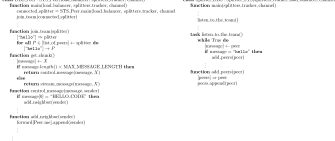
\includegraphics[width=\textwidth]{joining}
  \caption{Peer joining.\label{fig:joining}}
\end{figure*}
An incoming peer ${\cal P}_i$ (see the tasks described in
Fig.~\ref{fig:joining}) must contact a \emph{tacker} ${\cal R}$ to get
$[{\cal S}]$ in a \emph{reliable}\footnote{Reliable messages are
  transmitted over TCP and their transmission is denoted in the
  pseudocode by $\Rightarrow$. Unreliable messages, which can be lost
  in transit, are transmitted over UDP and its transmission is denoted
  by $\rightarrow$.} message. Then ${\cal P}_i$ polls sequentially
each splitter in $S$, requesting to be included in its team until one
of them (${\cal S}_j$, for example) accepts to ${\cal P}_i$. Then,
${\cal S}_j$ performs ${\cal T}_j = {\cal T}_j \cup {\cal P}_i$. In
parallel with the reception of $[{\cal T}_j]$, ${\cal P}_i$ sends a
(unreliable) $[\mathtt{hello}]$ to each ${\cal P}_k\in {\cal T}_j$,
and each ${\cal P}_k$ after the reception of the $[\mathtt{hello}]$
performs ${\cal T}_j = {\cal T}_j \cup {\cal P}_i$.
% When a ${\cal P}_k$ receives a $[\mathtt{hello}]$ from ${\cal P}_i$,
% replies to ${\cal P}_i$ with the same message. -> Ya no hace falta
% porque los peers van a calcular las rutas óptimas al resto de peers
% del team con el flooding con poda.
% _________________________________________________________________
% Cuando un peer llega al team, envía los hello's y comienza a recibir
% chunks. Los peers por defecto reenvían todos los chunks recibidos al
% resto de peers, excepto al que se lo ha enviado. Por cada chunk
% recibido duplicado, los peers envía a quien se lo ha envíado un
% mensaje de prunning con un peer origen (el que figura en el chunk
% duplicado), indicando que no le envíe más chunks con ese
% origen. Cuando un peer eche de menos un chunk de un determinado peer
% origen (un determinado número de veces), enviará a uno o varios
% peers (en pricipio a todos los peers) del team un mensaje de
% revocación de prunning, para asegurarse de que aparece una mejor
% ruta alternativa para ese peer origen.
% __________________________________________________________________
%Then, ${\cal P}_i$ computes the RTT (Round-Trip Time) for each
%$[\mathtt{hello}]$ reply, and does $T^*({\cal P}_i) = T^*({\cal P}_i) \cup
%{\cal P}_k$, for those peers which reply
%%for the $K$ peers with lowest RTT
%($T^*({\cal
%  P}_i)$ is, by definition, the \emph{reacheable} team of ${\cal
%  P}_i$).
%%Later, all ${\cal P}_k\in N({\cal P}_i)$ performs $N({\cal
%%  P}_k) = N({\cal P}_k) \cup {\cal P}_i$, when a chunk of stream is
%%received from ${\cal P}_i$.
% __________________________________________________________________
% Ya no hace falta
% __________________________________________________________________

\begin{comment}
$[{\cal L}]=[\{{\cal X}\in {\cal T}^0/|N({\cal
    X})|<K\}]$ (being $K$ the maximum connectivity degree and $N({\cal
  X})$ the neighborhood of ${\cal X}$), and after that, ${\cal S}^0$
adds ${\cal P}$ to ${\cal T}^0$. In parallel with the reception of
$[{\cal L}]$, ${\cal P}$ sends a $[\mathtt{hello}]$ message to each
$\{{\cal X}\in {\cal T}^0\}$. When a ${\cal X}$ receives a
$[\mathtt{hello}]$, replies to ${\cal R}$ with the same message. Then,
${\cal X}$ computes a $\text{RTT}({\cal X})$ (Round-Trip Time) for
each $[\mathtt{hello}]$ reply, and sends to the $K$ peers with lowest
RTT
%$\underset{{\cal P}_i^0\in X}{\operatorname{{\it K}-first~args~min}} \,
%\text{RTT}({\cal P}_i^0)=\{K\text{-first}~{\cal P}_i^0~|~\forall
%     {\cal P}_j\in X:\text{RTT}({\cal P}_j)\leq \text{RTT}({\cal
%       P}_i)\}$,
a $[\mathtt{neighborhood\_request}]$ message, which ${\cal X}$ must
reply with a $[\mathtt{neighborhood\_accept}]$, if ${\cal X}$ accepts
${\cal P}$ as a neighbor. For each found neighbor ${\cal X}$, ${\cal
  P}$ sends to ${\cal S}^0$ a $[\mathtt{neighborhood\_accepted}~{\cal
    X}]$, and ${\cal S}^0$ updates $N({\cal P}) = N({\cal P}) \cup
\{{\cal X}\}$.
\end{comment}

% Ungraceful leaves occur when a peer leaves the group without
% notice which may cause disconnection of the peer’s descendants
% from the group.

% Ungraceful exit made by a peer may cause interruption of data
% reception at its descendants.
\subsubsection{Leaving a team}
\label{dbs:leaving}
\begin{figure*}
  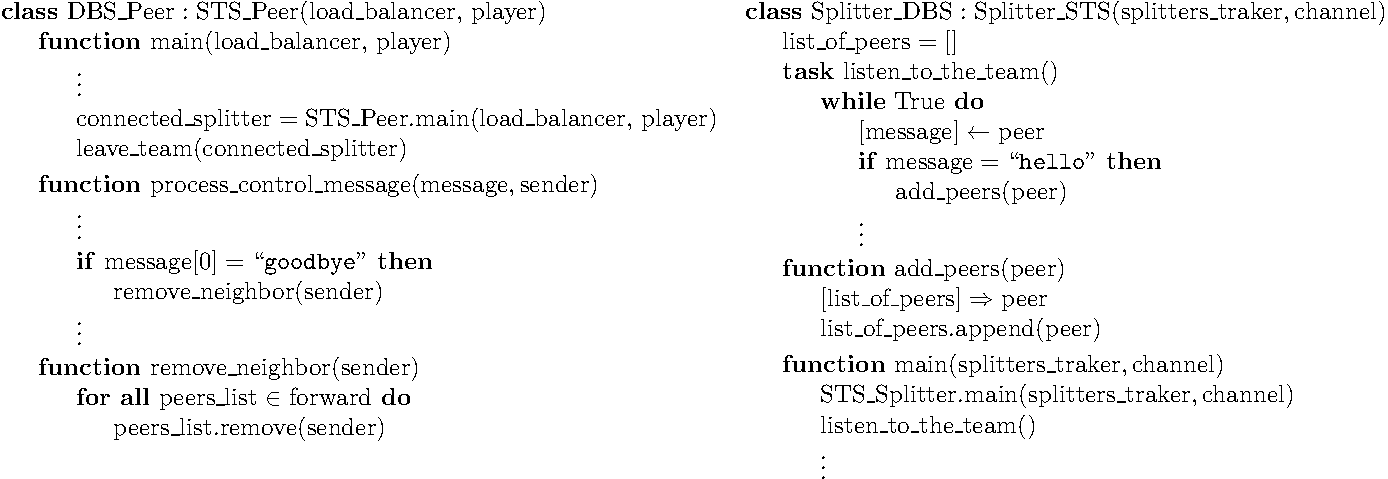
\includegraphics[width=0.55\textwidth]{leaving}
  \caption{Peer leaving.\label{fig:leaving}}
\end{figure*}
An outgoing peer ${\cal P}_o$ (see Fig.~\ref{fig:leaving}) from team
${\cal T}_j$ must to: (1) say $[\mathtt{goodbye}]$ to ${\cal S}_j$ and
to ${\cal T}_j$
%$N({\cal P}_o)$
(in this order), (2) relay any pending (received but
yet not sent) chunks, and (3) wait for a $[\mathtt{goodbye}]$ from
${\cal S}_j$, which performs ${\cal T}_j = {\cal T}_j \setminus {\cal
  P}_o$. In case of timeout, ${\cal P}_o$ resends the
$[\mathtt{goodbye}]$ and reset the leaving process, for a number of
times. When a ${\cal P}_k\in {\cal T}_j$
%${\cal P}_k\in N({\cal P}_i)$
receives a
$[\mathtt{goodbye}]$ from ${\cal P}_o$, ${\cal P}_k$ removes
%${\cal T}_j = {\cal T}_j \setminus {\cal P}_o$,
${\cal P}_o$ from the team.
%as a neighbor.
%, and finds the
%closest neighbor in ${\cal T}_j \setminus N({\cal X})$ by sending a
%$[\mathtt{hello}]$ to each of them and selecting the closest in terms
%of RTT (see \ref{dbs:joining}).

\begin{comment}
calls the Procedure \emph{Joining a
  team} (for $K=1$), to find a new neighbor. Finally, ${\cal S}_j$
sends to ${\cal P}_o$ a $[\mathtt{goodbye}]$ and performs ${\cal T}_j
= {\cal T}_j \setminus \{{\cal P}_o\}$.
\end{comment}

\subsubsection{Chunk generation}
\label{dbs:chunk_generation}
\begin{figure*}
  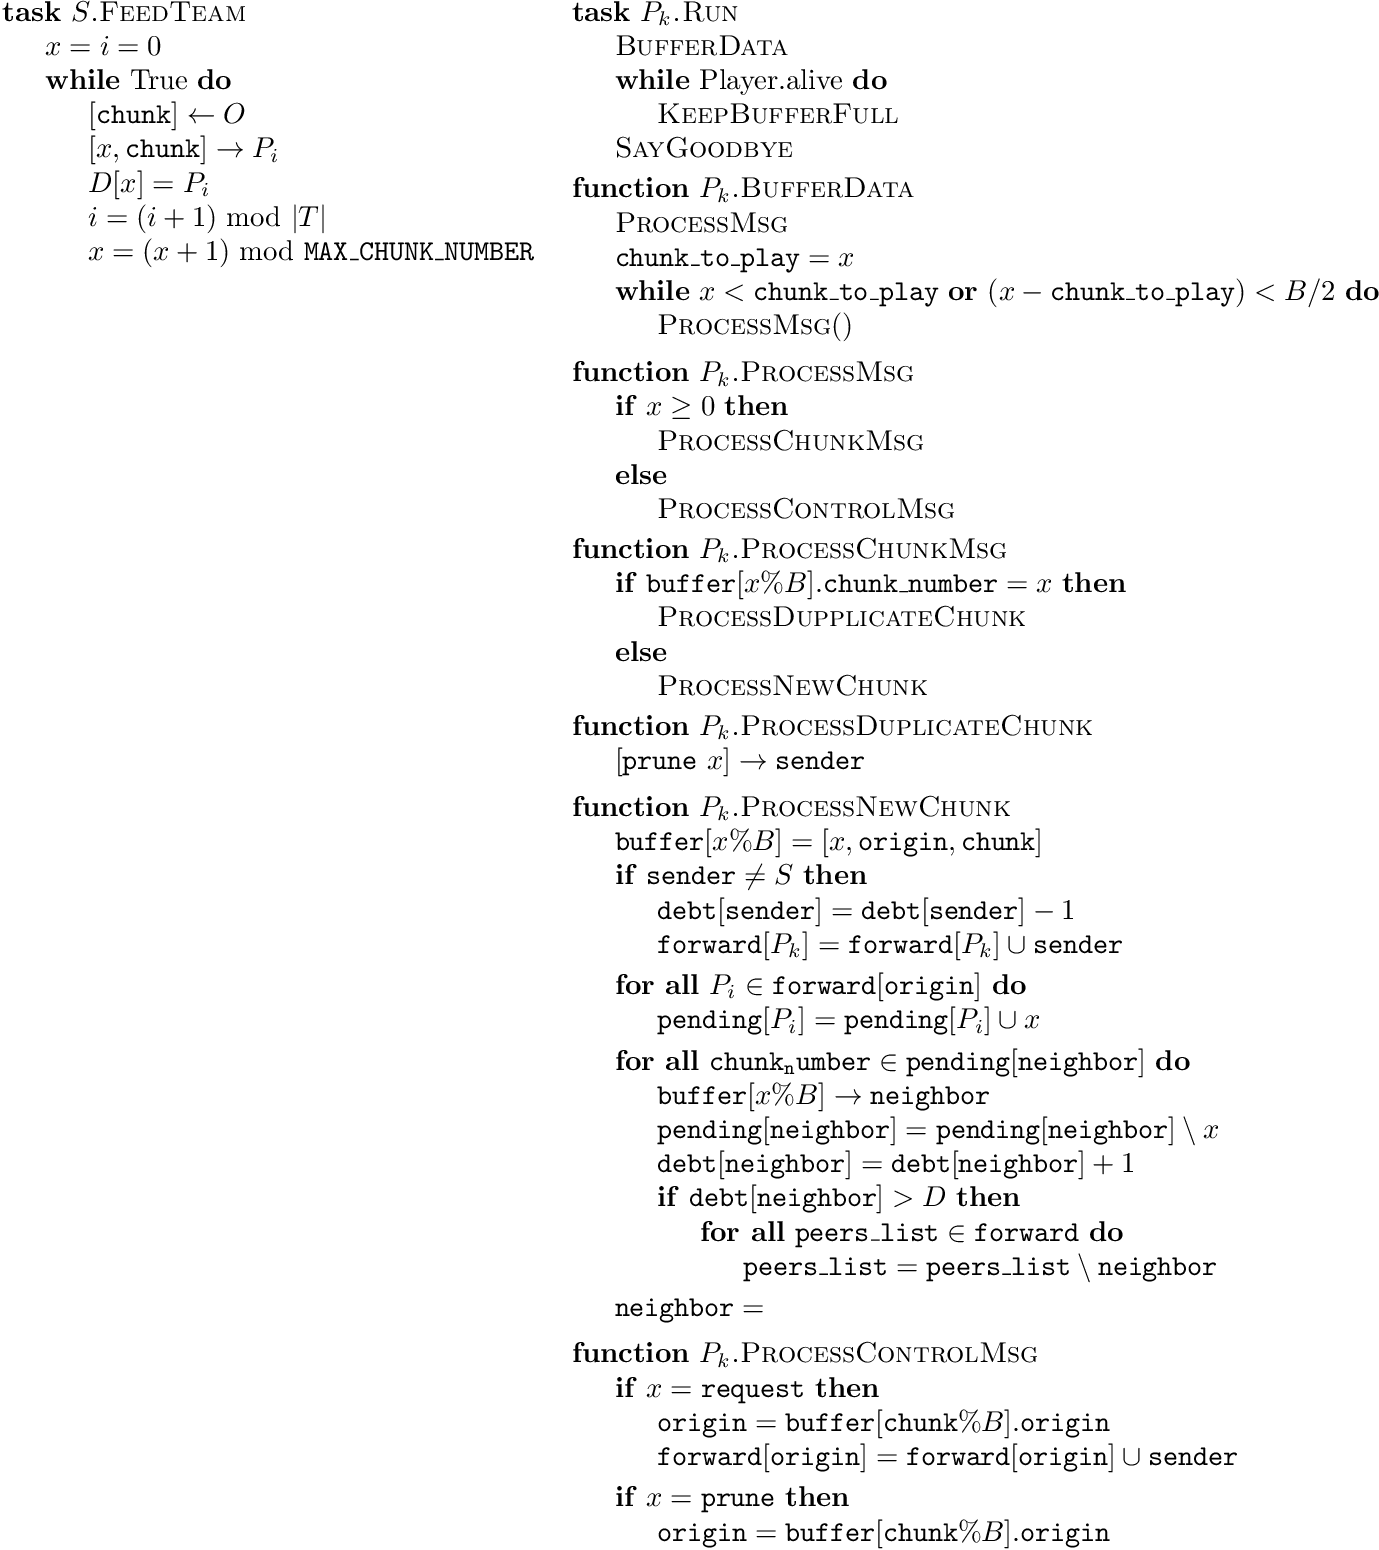
\includegraphics[width=0.75\textwidth]{chunk_generation_and_flooding}
  \caption{Chunk generation and
    flooding.\label{fig:chunk_generation_and_flooding}}
\end{figure*}
Each ${\cal S}_j\in{\cal S}$ (see
Fig.~\ref{fig:chunk_generation_and_flooding}) divides the stream into
chunks of data ($\mathtt{chunk}$) of constant length $C$ (and
identical content among teams), and sends exclusively each chunk to a
different \emph{origin peer} ${\cal P}_i\in{\cal T}_j$, using a
round-robin schema. Each chunk is enumerated with a index $x$, forming
the message $[c_x]=[x,\mathtt{chunk\_data}]$, where
$x=i~\mathrm{mod}~|{\cal T}_j|$. We define a \emph{round} (in a team)
as the time necessary to send two consecutive chunks from the splitter
(of such team) to the same peer. This time is variable and depends on
$|{\cal T}_j|$, $C$, and the average bit-rate of the media, $R$.

\begin{comment}
The round-time is defined by:
\begin{equation}
  \cal{r} = \cal{c}N.
  \label{eq:round_time}
\end{equation}
For example, if we use only one team of $N=256$ peers, a chunk size
$C=1024$~bytes, and a video of $1$~Mb/s, the round time is
\begin{displaymath}
  \cal{r} = \frac{1024\frac{\text{bytes}}{\text{chunk}}\times
    8\frac{\text{bits}}{\text{byte}}}{10^6\frac{\text{bits}}{\text{second}}}\times
  256 \approx 2.1~\text{seconds}.
\end{displaymath}
\end{comment}

\subsubsection{Chunk flooding}
\label{dbs:chunk_flooding}
When peers receive chunks, flood them to the rest of peers of the team
(except to the sender), using again a round-robin schema (see
Fig.~\ref{fig:chunk_generation_and_flooding}). For each duplicate
chunk received by a ${\cal P}_k \in {\cal T}_j$ from ${\cal P}_l \in
{\cal T}_j$, ${\cal P}_k$ sends to ${\cal P}_l$ a
$[\mathtt{prune}~{\cal P}_i]$, where ${\cal P}_i$ is the origin peer
of the duplicate chunk. Thus, only the first ${\cal P}_l$ to send to
${\cal P}_k$ a chunk ``originated'' at ${\cal P}_i$ will do that in
the future, at least that ${\cal P}_k$ revokes this routing
information by sending a $[\mathtt{not~prune}~{\cal P}_i]$ to one or
more (possibly the rest of) peers of the team.

%When peers receive chunks from their splitter, they must flood them to
%their neighbors until the chunks are broadcasted to the whole team
%(Fig.~\ref{fig:chunk_generation_and_flooding}). Lets suppose that
%${\cal P}_k$ receives a chunk. In the case the sender is its splitter,
%${\cal P}_k$ floods the chunk to $N({\cal P}_k)$. However, if the
%sender is a peer ${\cal P}_m\in N({\cal P}_k)$, ${\cal P}_k$ adds
%${\cal P}_m$ to $N({\cal P}_k)$ if ${\cal P}_m$ is a new neighbor, and
%forwards the chunk to the rest of its neighborhood ${\cal P}_n\in
%N({\cal P}_k)\setminus{\cal P}_m$ if ${\cal P}_k$ is in the shortest
%between ${\cal P}_n$ and the origin peer ${\cal P}_i$ of the relayed
%chunk. This will be true if ${\cal P}_k$ is the gateway of ${\cal
%  P}_n$ to go from ${\cal P}_n$ to ${\cal P}_i$. Therefore, a flooding
%with prunning based on shortest path routing is used.

\subsubsection{Chunk buffering}
In order to hide the jitter generated by the physical network and
P2PSP, peers store the received chunks before playing them. A chunk
$c_x$ is inserted in the position $(x~\mathit{mod}~B)$ of the buffer,
being $B$ the buffer size in chunks and ``$\mathit{mod}$'' the modulo
operator. A chunk is given by lost when it is time to send it to the
player and the chunk has not been received.

\begin{comment}
\subsubsection{Shortest path computation}
\label{dbs:chunk_routing}
\begin{figure}
  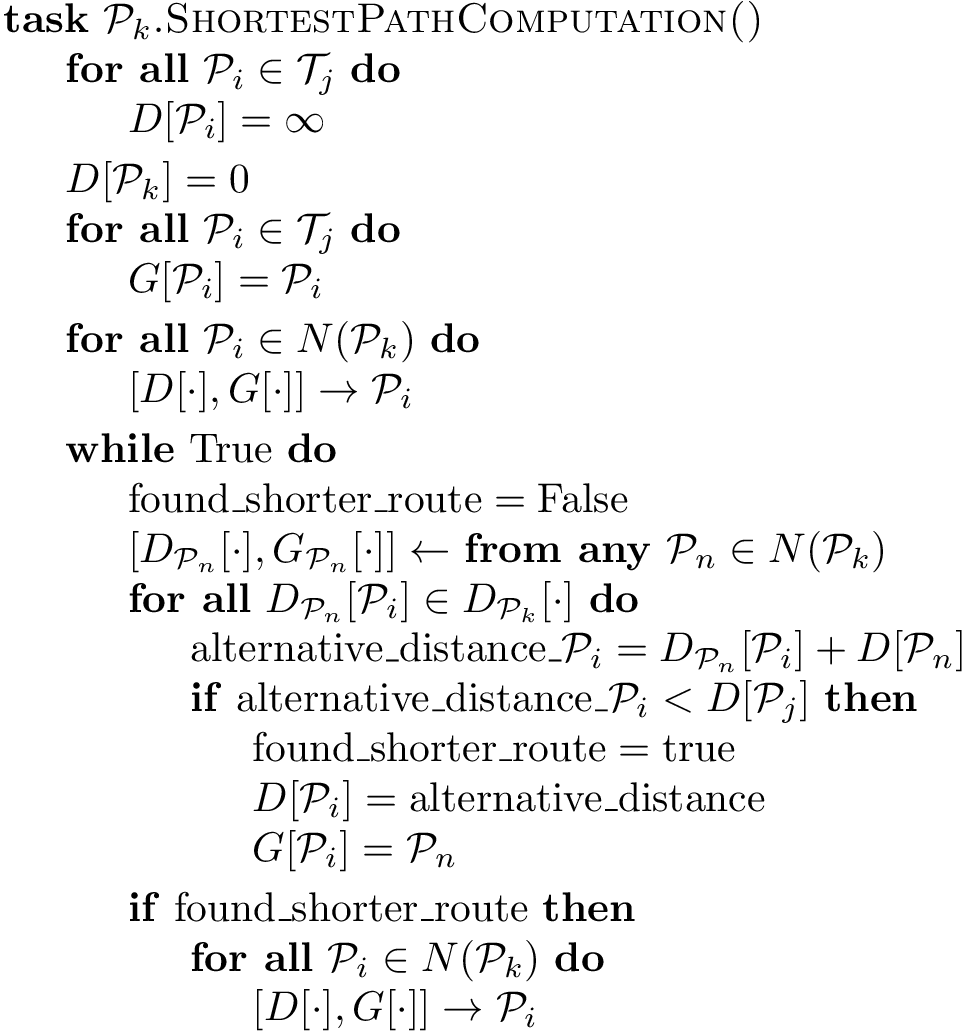
\includegraphics[width=0.35\textwidth]{shortest_path_computation}
  \caption{Shortest path computation.\label{fig:shortest_path_computation}}
\end{figure}
The shortest path distances among peers are determined by a variation
of the Bellman-Ford Algorithm~\cite{Bertsekas1987data} (see
Fig.~\ref{fig:shortest_path_computation}), where the cost of the
``links'' between neighbor peers is $1$. Neighbor peers interchange
two vectors $D[\cdot]$ (distance-to-peer) and $G[\cdot]$
(gateway-to-peer) and compute the shortest distances and the (peer)
gateways to (reach) the rest of peers of its team ${\cal T}_j$.

This algorithm is free of routing loops and is not suceptible of the
well known count-to-infinity problem, and therefore always converges
for static teams. These problems do not appear because the routes are 

Each peer ${\cal P}_k$ sends
its vector of distances $D[\forall {\cal P}_i\in T^*({\cal P}_k)]$ and
gateways $G[\forall {\cal P}_i\in T^*({\cal P}_k)]$ to each
neighbor. When this information is received, peers check if shorter
routes can be found to the rest of peers of the reachable team, and if
so, send these vectors again.

The Bellman-Ford algorithm is susceptible of routing loops and the
count-to-infinite problem.


% Hace falta saber desde dónde viene el chunk original (origin peer) y que todos los peers dispongan de los vector-distances de los peers vecinos. Los vector-ditances deben tener tantas entradas como peers existen en el team. Por tanto, cada peer almacena un número de vector-distances igual a su grado de conectividad.


% Supposing that the weight of links between neighbors is 1.
% ¿Cómo sabe un peer que él es el último?
\end{comment}

\begin{comment}
\subsubsection{Generation of the routing tables}
Routing tables has as many entries as peers are in the team. The
routing table of a peer $P_i$ is a dictionary of pairs ($d(P_i, P_j)$,
$P_k$) indexed by the destination peer $P_j$ is a destination peer,
where $d(P_i, P_j)$ is the last measurement of the number of hops (in
peers) between $P_i$ and $P_j$, and $P_k\in N(P_i)$ is the 1-hop peer
that in the shortest-path between $P_i$ and $P_j$. Notice that if
$P_j==P_k$ then $d(P_i, P_j)==1$, which means that $P_i$ and $P_j$ are
directly ``connected''.

When a peer has updated its routing table, it is sent to their
neighbors pyggibacked on a \textsf{chunk} packet. When a peer receives
a routing table, it keeps a copy of it and updates its own routing
table with the new routing information using the Bellman-Ford
Algorithm~\cite{}. The peers have a copy of the routing table of its
neighbors to use it through the chunk routing process (see
Rule~\cite{the_routing_process}.
\end{comment}

\subsubsection{Free-riding control at splitters}
\label{dbs:frcS}
In each team there are a set of peer \emph{monitors} (trusted peers
whose behavior is predictable), which complain to their splitter when
a chunk is lost. Lets suppose that chunk $c_x$ was sent to ${\cal
  P}_i\in {\cal T}_j$. If ${\cal S}_j$ receives a
$[\mathtt{lost\_chunk}~x]$ from each monitor of ${\cal T}_j$, and if
this happens during $L$ consecutive rounds, ${\cal S}_j$ considers
that ${\cal P}_i$ has leaved ${\cal T}_j$, and removes it from the
team.

\subsubsection{Free-riding control at peers} % Neighborhood dynamics
\label{dbs:frcp}
In each round, peers check if a chunk have been received from the rest
of peers of the team (${\cal P}_k\in {\cal T}_j)$). If not, peers send
a $[\mathtt{not~prune}~{\cal P}_i]$ to one or more (possibly
to the rest of) peers of the team, where ${\cal P}_i$ is the origin peer
of the missing chunk. At this point, the process continues as
described in Section~\ref{dbs:chunk_flooding}.

\begin{comment}
For each ${\cal P}_k\in N({\cal P}_i)$, ${\cal P}_i$ checks if a chunk
has been received from ${\cal P}_k$. If ${\cal P}_i$ detects that
${\cal P}_k$ has not sent a chunk to it during $L$ consecutive rounds,
performs $N({\cal P}_i) = N({\cal P}_i)\setminus{\cal P}_k$, and stops
sending to ${\cal P}_k$ more chunks.
\end{comment}
\begin{comment}
computes a
``chunk-debt'', denoted by $d({\cal P}_k)$, that is incremented each
time a chunk is received from ${\cal P}_k$ and decremented each time a
chunk is sent to ${\cal P}_k$. If ${\cal P}_i$ verifies that $d({\cal
  P}_k)>D$ (the maximum debt), then ${\cal P}_i$ considers that ${\cal
  P}_k$ is unable to communicate with it, performs $N({\cal P}_i) =
N({\cal P}_i)\setminus{\cal P}_k$, and stops sending to ${\cal P}_k$
more chunks.
\end{comment}

\subsubsection{Congestion control}
\label{dbs:congestion_control}
P2PSP is a content-unaware push-based protocol. To avoid network
congestion while flooding, sending peers must perform some kind of
data flow-control. Moreover, to achieve aN ideal I/O ratio of $1$,
peers should send one chunk for every received one.

Congestion control in P2PSP is very simple: if a new chunk is
received, peers forward (using the flooding with prunning algorithm
described in Sec~\ref{dbs:chunk_generation_and_flooding}) each
received chunk to the next peer of their list of peers (following a
round-robin pattern).

%Peers do not understand the content, but it is
%known that in order to achieve a I/O ratio of 1, peers should send one
%chunk for every received one, on average. To acomplish this, a ${\cal
%  P}_i$ creates a FIFO queue of chunks for each $N({\cal P}_i)$, and,
%for each received chunk, ${\cal P}_i$ forwards a queued chunk from
%each of these queues.

\begin{comment}
A ${\cal P}_i$ forwards one or more chunks if and only if it has
received a chunk. For each received chunk $c_j$, ${\cal P}_i$: 1)
creates a list $l_{c_j}$ with the contents of $N'({\cal P}_i)$, and 2)
sends $c_j$ to $l_{c_j}[0]$ (the first element), and removes
$l_{c_j}[0]$. For each chunk reception, Step 2) is repeated for all
the previously created lists while they are not exhausted.

A solution is a forwarding algorithm based on the following
idea. Peers manage a list of chunks, where every item is a 2-tuple
($c_k$, $P_l$). The field $c_k$ represents the chunk that must be
flooded (if the node that has delivered the chunk is the splitter,
$c_k$ must be relayed towards all the neighbors, otherwise, $c_k$ must
be sent to all the neighbors except the peer that delivered $c_k$),
and the field $P_l$ the last neighbor to which $c_k$ was sent. For
every chunk received, a new tuple is appended to the list of chunks
and the rest of tuples are updated. The field $c_k$ remains constant
but $P_l$ is replaced by the next peer in the list of neighbors for
every received chunk.
\end{comment}

\begin{comment}
\subsubsection{Flooding order}
\label{dbs:flooding_order}
As an incentive mechanism~\cite{xu2006analysis}, peers relay received
chunks first to those peers that 
\end{comment}

%neighbors with lower chunk-debts.

\begin{comment}
\subsubsection{Team dynamics}
\label{dbs:team_dynamics}
${\cal P}_i$ adds to $N({\cal P}_i)$ those ${\cal P}_j$ that has sent
to ${\cal P}_i$ a chunk. If $N({\cal P}_i)>K$, periodically, ${\cal
  P}_i$ removes from $N({\cal P}_i)$ the peer with highest chunk-debt
and try to find in ${\cal T}_j\setminus N({\cal P}_i)$ a new peer using
$[\mathtt{hello}]$ messages.
\end{comment}

\begin{comment}
Peers use a buffer $b$ of chunks to hide the jitter generated by the
physical network and the broadcasting protocol. When a peer receives
$C_i$, it performs
\begin{equation}
  b[i~\text{mod}~B] = c_i,
\end{equation}
where ``mod'' represents the modulo operator and $B$ the buffer size
(in chunks). Basically, the buffer represents a sliding window that
moves over the stream synchronizely with the playing because the the
player consumes the chunks at the same chunk-rate the source produces
them.
\end{comment}

%%%%%%%%%%

\begin{comment}

\begin{itemize}

\item In the P2PSP, only monitor peers complains about lost
  chunks. This means that if a chunk that has been retransmitted by a
  peer is lost, it will be only retransmitted to all the peers of the
  team if the destination is a monitor peer and there is a unique
  monitor peer in the team. On the other hand, if the lost chunk was
  traveling from the splitter to a peer, all monitor peers will
  complain and this chunk will be retransmitted to the complete
  team. Therefore, only massively loss chunks will be retransmitted in
  the P2PSP. However, notice that a isolated missing chunk will
  produce negligible artifacts in the playback of one peer. In the
  Chain model, the lost of a chunk is handled between neighbour peers
  which means that all lost blocks should be, a priori, recovered.

\end{itemize}

%}}}

\end{comment}
